\documentclass[12pt]{article}

\usepackage{sbc-template}
\usepackage{graphicx,url}
\usepackage[latin1]{inputenc}  

\usepackage{../Utils}
     
\sloppy

\title{The Implementation of Proxima \\{\small \version}}

\author{Martijn M. Schrage\inst{1}}


\address{Institute of Information and Computing Sciences\\ Utrecht University\\
    Utrecht, The Netherlands
  \email{martijn@cs.uu.nl}
}

\begin{document} 

\maketitle

\begin{abstract}

~\\ \bl
\o Generic editor as IDE
\o Implementation of Proxima 
\el

\end{abstract}
     


\section{Introduction}
Proxima~\cite{schrage04Proxima}.

\begin{figure}[ht]
\centering
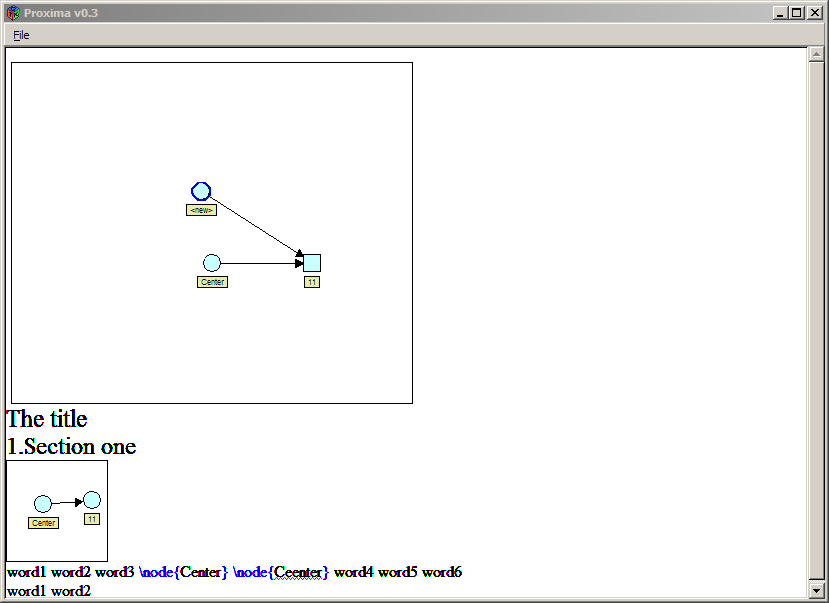
\includegraphics[width=\textwidth]{images/screenshots/BayesDocEditor}
\caption{The Bayesian network documentation editor}
\label{fig:bayesEditor}
\end{figure}

\section{Presenting}
\section{Xprez}
\section{Scanning}
\section{Parsing}
\section{Incrementality}
\section{Conclusion} 

% refs: Section~\ref{sec:figs}  Figure~\ref{fig:exampleFig1}



\bibliographystyle{sbc}
\bibliography{../proxima}

\end{document}
